\documentclass[envcountsect, smaller, aspectratio=149]{beamer}
\usetheme[headheight=0em, logo=none, themepath=beamercolorthemefibeamer, nofonts]{fibeamer}
\usepackage{beamercolorthemefibeamer}
\setbeamerfont{frametitle}{size=\large}
\usepackage[utf8]{inputenc}
\usepackage[english, ngerman]{babel}
\usepackage{caption}
\captionsetup{justification=centering}
\bibliographystyle{abbrv}


\title{Neuronale Faltungsnetze und Pooling}
\author{Michael Markl\\25. Juni 2021}
\date{25. Juni 2021}
\subtitle{Mathematische Aspekte des Maschinellen Lernens\\
Seminar bei Prof. Dr. Stykel}
\begin{document}

\maketitle

\begin{frame}{Experiment von Hubel und Wiesel~\cite{Hubel1959, Hubel1962}}
    
\begin{figure}
    \vspace*{-2em}
    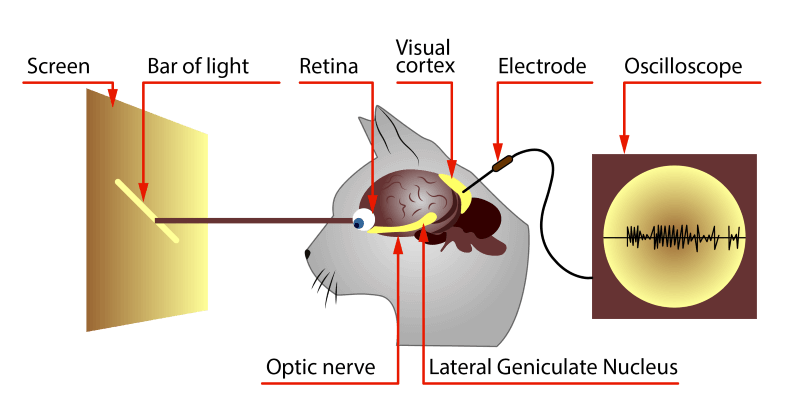
\includegraphics[width=0.8\textwidth]{cat-experiment.png}
    \vspace{-1em}
    \caption{Messung der Aktivität einzelner Neuronen des visuellen Cortex bei Licht-Reizen. {\scriptsize(Grafik aus~\cite{Ver17})}}
\end{figure}

\end{frame}

\begin{frame}{Drei Kernresultate des Experiments}

\begin{minipage}[t]{1.05\textwidth}
    \begin{itemize}
    \onslide<2->\item Jedes Neuron hat ein \textbf{lokales rezeptives Feld},
        d.\,h. es reagiert nur auf Reize aus einer kleinen Umgebung des Ursprungsbildes.
    \onslide<3->{\item Auf dem rezeptiven Feld hat das Neuron \textbf{erregende} (engl. excitatory) \textbf{und} \textbf{hemmende} (engl. inhibitory) \textbf{Regionen}.}
    \onslide<4->{\item Der visuelle Cortex ist in Spalten aufgebaut.
    Neuronen \textbf{tieferer Schichten} nutzen als Rezeptoren die Aktivierung von Neuronen der Schicht darunter und erkennen \textbf{komplexere Strukturen}.}
\end{itemize}
\end{minipage}

\vspace{0.5em}
\begin{minipage}[c]{0.5\textwidth}
    \onslide<2->{
    \begin{figure}
        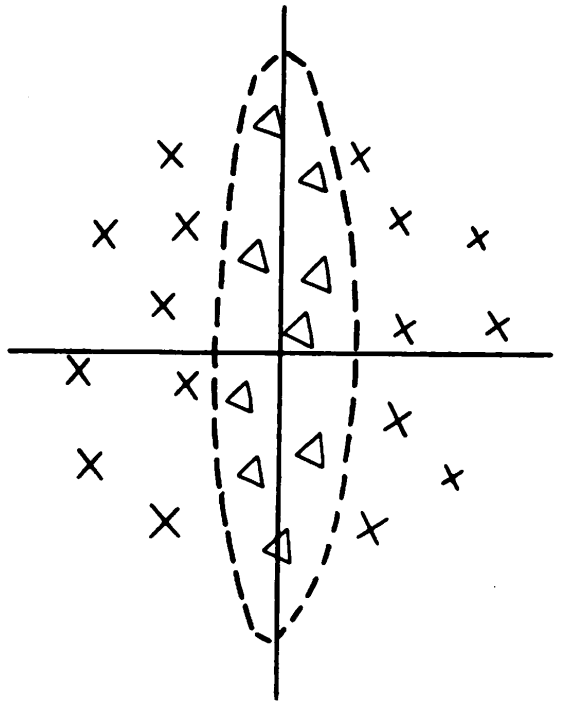
\includegraphics[width=0.35\textwidth]{receptive-field-cat.png}
        \vspace{-0.5em}
        \caption{Rezeptives Feld eines Neurons.\\$x$: erregend; $\Delta$: hemmend. {\scriptsize (Grafik~aus~\cite{Hubel1959})}}
    \end{figure}
    }
\end{minipage}%
\begin{minipage}[c]{0.5\textwidth}
    \onslide<4->{
    \begin{figure}
        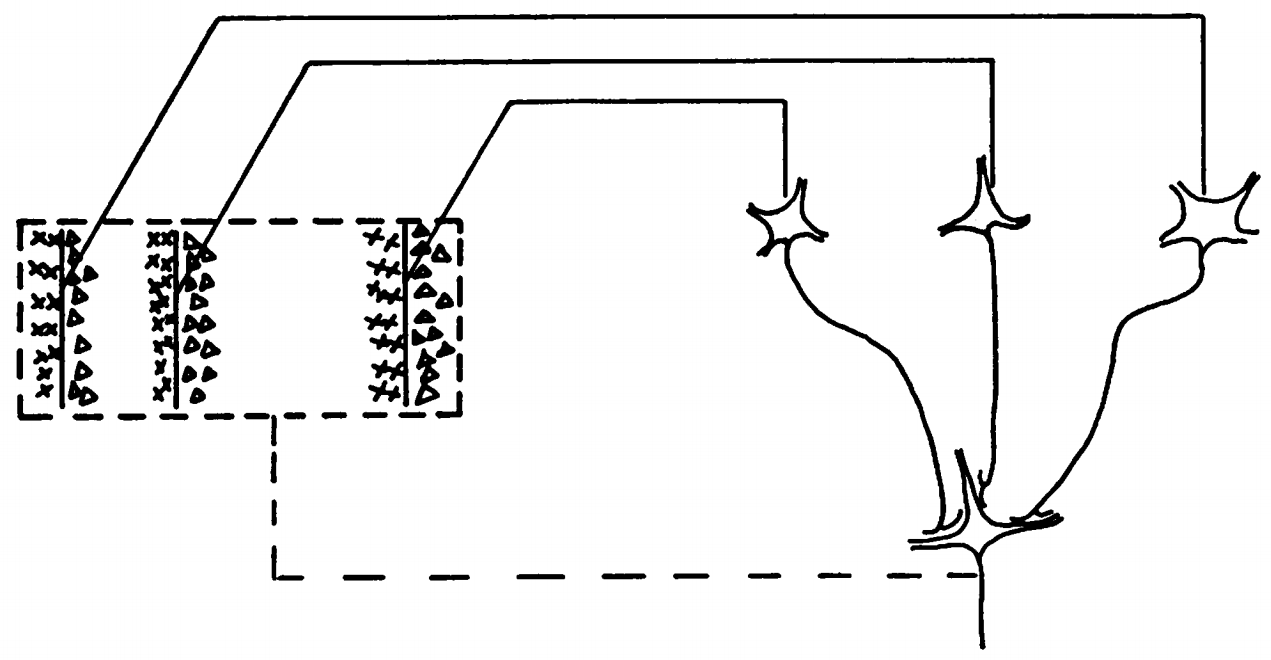
\includegraphics[width=0.86\textwidth]{complex-cells.png}
        \vspace{-0.5em}
        \caption{Aufbau komplexer Zellen {\scriptsize (Grafik~aus~\cite{Hubel1962})}}
    \end{figure}
    }
\end{minipage}

\end{frame}

%%%%
% Hubel und Wiesel haben dafür 1981 den Nobel-Preis erhalten.

\section*{ }

\begin{frame}<presentation:0>[noframenumbering]
    \cite{Calin2020}
    \cite{Goodfellow-et-al-2016}
\end{frame}

\begin{frame}{Literatur}
	\scriptsize
	\bibliography{literature}
\end{frame}

\end{document}